\subsection{Main Results}
\label{sec:main-results}

\subsubsection{Candidate Ceiling and Reranking Gains}

Before any reranking, we need to know how much evidence is even reachable. The original Hybrid RRF posts test Recall@100 of 0.6077, meaning roughly 40\% of gold passages never enter the candidate pool. The enhanced w122 configuration lifts this ceiling to 0.7388 (Figure~\ref{fig:recall-at-k}), adding over 13 percentage points of recoverable evidence.

\begin{figure}[t]
\centering
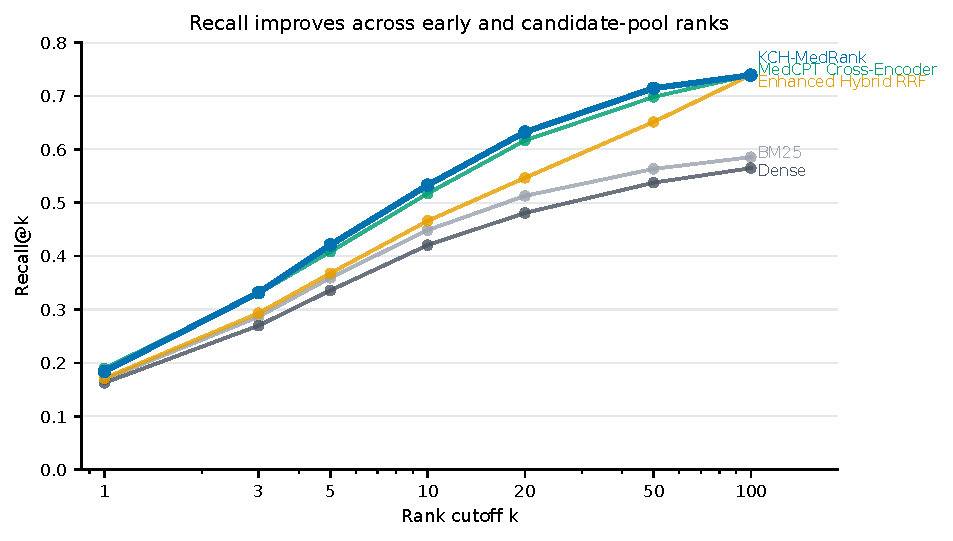
\includegraphics[width=0.98\linewidth]{figures/data_figures/fig3_recall_at_k.pdf}
\caption{Recall@$k$ curves on the held-out BioASQ split. KCH-MedRank improves early-rank evidence coverage while sharing the enhanced top-100 candidate ceiling with the MedCPT Cross-Encoder and enhanced Hybrid RRF.}
\label{fig:recall-at-k}
\end{figure}

KCH-MedRank then reorders within this larger pool to reach Recall@10 of 0.5329 against 0.4660 for the enhanced Hybrid RRF ordering (Figure~\ref{fig:main-results}). The $\Delta$ of $+0.0669$ translates to roughly one additional gold passage entering the top 10 for every 15 questions. MRR@10 moves from 0.7530 to 0.7867 and nDCG@10 from 0.5843 to 0.6433. All four top-10 metrics are significant under paired bootstrap ($p=0.0002$).

\begin{figure*}[t]
\centering
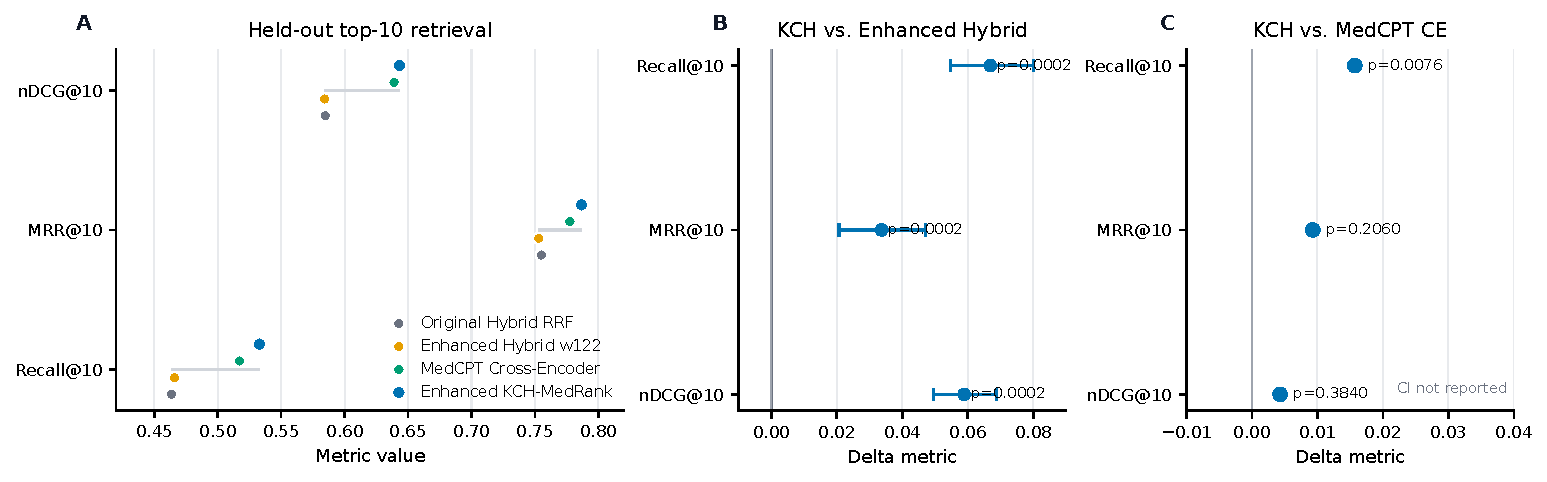
\includegraphics[width=0.98\textwidth]{figures/data_figures/fig2_main_results.pdf}
\caption{Main BioASQ results and confirmatory comparisons. Panel A compares top-10 retrieval metrics across the main methods. Panel B shows paired-bootstrap deltas for KCH-MedRank over enhanced Hybrid RRF with 95\% confidence intervals. Panel C shows KCH-MedRank over the MedCPT Cross-Encoder; confidence intervals are not reported in the source table, so only point estimates and $p$-values are shown.}
\label{fig:main-results}
\end{figure*}

\subsubsection{Beating the Cross-Encoder}

The stricter test is the MedCPT Cross-Encoder, which scores each query-passage pair through a full transformer. On the same enhanced candidate pool it reaches Recall@10 of 0.5172. KCH-MedRank improves on this by $+0.0157$ ($p=0.0076$, paired bootstrap; Figure~\ref{fig:main-results}C). MRR@10 and nDCG@10 are positive at $+0.0092$ and $+0.0043$ but not significant.

Significant recall gains without significant MRR movement make sense for evidence retrieval. Recall checks whether relevant passages appear anywhere in the top 10. MRR checks whether the first passage is relevant. KCH-MedRank lifts evidence that semantic scoring alone pushed just outside the top-10 window. It does not need to reshuffle passages that are already well-ranked to improve coverage.

\subsubsection{Rescuing Hard Cases}

The hard subset isolates 65 questions where the candidate pool holds gold evidence but the top 10 contains none (Table~\ref{tab:hard-subset-diagnostic}). By construction, enhanced Hybrid RRF has Recall@10 of 0 here. KCH-MedRank pulls gold evidence into the top 10 for nearly half of these questions (Recall@10 = 0.4704). Retrieval-feature-only LambdaMART reaches 0.4411. The gap of $+0.0293$ between them is the incremental value of biomedical knowledge features on questions that retrieval signals alone leave untouched.

\begin{table}[t]
\centering
\small
\caption{Diagnostic hard reranking subset on held-out BioASQ questions where enhanced Hybrid top-100 contains gold evidence but enhanced Hybrid top-10 misses it.}
\label{tab:hard-subset-diagnostic}
\begin{tabular}{lrrrr}
\toprule
Method & Recall@10 & MRR@10 & nDCG@10 & Recall@100 \\
\midrule
Enhanced Hybrid RRF & 0.0000 & 0.0000 & 0.0000 & 0.8375 \\
Retrieval-feature-only LambdaMART & 0.4411 & 0.2180 & 0.2424 & 0.8375 \\
Flat knowledge LTR, no graph & 0.4550 & 0.2855 & 0.2907 & 0.8375 \\
Pairwise graph LTR & 0.4508 & 0.2725 & 0.2766 & 0.8375 \\
Full KCH-MedRank & 0.4704 & 0.2836 & 0.2945 & 0.8375 \\
\bottomrule
\end{tabular}
\end{table}


\subsubsection{Generalization}

PubMedQA tests whether the approach transfers to a different QA format (Table~\ref{tab:pubmedqa-retrieval-diagnostic}). The lightweight HGB knowledge reranker lifts Recall@10 from 0.8200 to 0.8953 over its Hybrid RRF source ($p=0.0002$). MRR@10 barely moves (0.9850 to 0.9861). This mirrors BioASQ: the method expands evidence coverage without touching already-strong first-rank precision. We note that this transfer uses a lightweight HGB reranker, not the complete BioASQ KCH-MedRank pipeline.

\begin{table}[t]
\centering
\small
\caption{Secondary PubMedQA retrieval diagnostic on the held-out test split. The HGB knowledge reranker is a lightweight robustness reranker over the Hybrid candidate pool, not the main enhanced BioASQ KCH-MedRank configuration.}
\label{tab:pubmedqa-retrieval-diagnostic}
\begin{tabular}{lrrrr}
\toprule
Method & Recall@10 & MRR@10 & nDCG@10 & Recall@100 \\
\midrule
BM25 & 0.7284 & 0.9510 & 0.7490 & 0.8526 \\
Dense & 0.8644 & 0.9863 & 0.8760 & 0.9425 \\
Hybrid RRF & 0.8200 & 0.9850 & 0.8369 & 0.9350 \\
Cross-encoder rerank & 0.8268 & 0.9806 & 0.8381 & 0.9410 \\
HGB knowledge reranker & 0.8953 & 0.9861 & 0.9021 & 0.9350 \\
\bottomrule
\end{tabular}
\end{table}


BEIR NFCorpus tests the supervised reranking layer in isolation, since MeSH, entity, PrimeKG, and hypergraph features are not built there (Table~\ref{tab:nfcorpus-retrieval-diagnostic}). Retrieval-feature LambdaMART improves Recall@10 from 0.1676 to 0.1770 ($p=0.0034$) and nDCG@10 from 0.3436 to 0.3627 ($p=0.0002$) over Hybrid RRF. This confirms that listwise supervised reranking generalizes beyond BioASQ even without domain-specific knowledge features. Full KCH-MedRank generalization, including biomedical knowledge and hypergraph features, remains to be tested on datasets where such features can be constructed.

\begin{table}[t]
\centering
\small
\caption{External BEIR NFCorpus retrieval-only diagnostic on the official test split. The LambdaMART row uses only BM25, dense, Hybrid RRF, score, and rank features; it does not use NFCorpus-specific MeSH, entity, PrimeKG, or hypergraph features.}
\label{tab:nfcorpus-retrieval-diagnostic}
\begin{tabular}{lrrrr}
\toprule
Method & Recall@10 & MRR@10 & nDCG@10 & Recall@100 \\
\midrule
BM25 & 0.1379 & 0.5063 & 0.2933 & 0.2228 \\
Dense & 0.1674 & 0.5399 & 0.3496 & 0.3096 \\
Hybrid RRF & 0.1676 & 0.5530 & 0.3436 & 0.3242 \\
Retrieval-feature LambdaMART & 0.1770 & 0.5725 & 0.3627 & 0.3242 \\
\bottomrule
\end{tabular}
\end{table}

